\taskpic{C одним молем идеального одноатомного газа провели замкнутый
цикл, изображённый на рисунке, где $1-2$ изотерма, $2-3$ изобара,
$3-4$ политропа, для которой $C = R/2$, и $4-1$ изохора. Минимальная
температура, достигаемая газом в цикле, $T_{min} = 300 \,
К$. Политропическим процессом называется процесс, происходящий с
постоянной теплоёмкостью $C$. Определите КПД цикла
$\eta$.}{
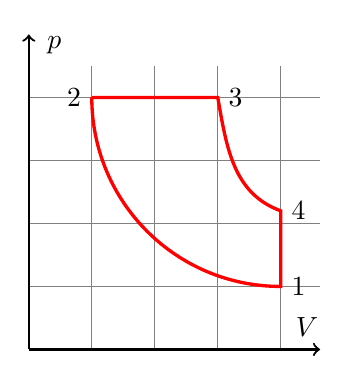
\begin{tikzpicture}
  \draw[help lines,step=0.8] (0,0) grid (3.7,3.6);  
  \draw[thick,->] (0,0) -- (3.7,0) node [above=8,left=-3] {$V$};
  \draw[thick,->] (0,0) -- (0,4) node[above=-4,right=3] {$p$};
  \draw[very thick,red] (0.8,3.2) node[black,left] {2} -- (2.4,3.2)
  node[black,right] {3} to[out=-80,in=160]
  (3.2,0.8*2.2) node[black,right] {4} -- (3.2,0.8) node[black,right] {1} to [out=180,in=-90]
  (0.8,3.2);
\end{tikzpicture}
}
